\chapter{Technical Approach}

\section{Background}
\subsection{Data-flow Analysis}
In compiler theory, data-flow analysis is a technique for gathering information about the possible set of values calculated at various points in a computer program. The basis for performing data-flow analysis is control flow graph (CFG), which is used to determine those parts of the program to which a particular value assigned to a variable might propagate. In our particular case, we used reaching-definition for each instruction to represent the data flow information. Two techniques applied for performing reaching-definition analysis are \textit{Liveness Analysis} and \textit{Reaching-Def Analysis}.

%CFG and ICFG
Control Flow Graph (CFG) is a graph representation of all the paths that a computer program might be traversed through during its execution. In a control flow graph, each node represents a basic block - a sequencial piece of a program that does not include jumps or jump targets, while the directed edges represent jumps in the program. Figure 2.1 is the complete control flow graph constructed for an example function t3f1. Each circle represents a basic block (first number in the circle denotes its line number), and the black edges represent the possible jumps that the program can take during execution. It is worth noting that the while loop in t3f1 includes a condition check at line 4, which can be reached from either line 4 (before loop starts) or from line 13 (after last instruction in the loop is finished). Therefore in the CFG there are two nodes representing line 5, with one coming from line 4 and another coming from line 13.

\begin{figure}
\begin{minipage}{\textwidth}
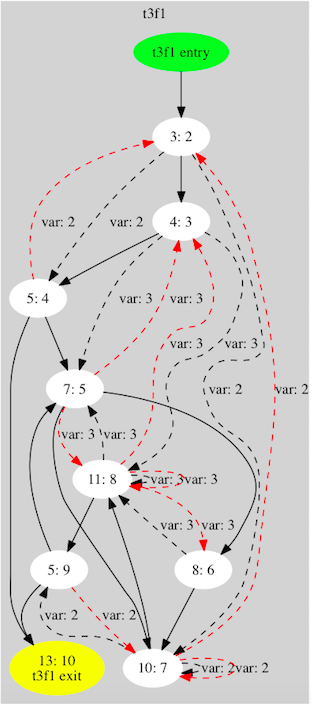
\includegraphics[width=0.6\textwidth]{figures/CFG.png}
\caption{Control Flow Graph for Function t3f1}
\label{CFG}
\end{minipage}
\end{figure}

\lstset{language=PHP}
\begin{minipage}{0.5\textwidth}
\begin{lstlisting}[frame=single]
<?php
function t3f1($c, $d) {
  $a = 0;
  $b = 0;
  while($a <= 5)
  {
    if ($b > 5) {
      $b = 5;
    }
    $a = $a + 1;
    $b = $b + 2;
  }
}
?>
\end{lstlisting}
\end{minipage}
\newline

%liveness analysis and reaching-def analysis
As one of the two techniques used for performing reaching-definition analysis, liveness analysis is to calculate, at instruction level, the variables that may be potentially read before their next write, that is, the variables that are live at the exit from each program point. In the given example, variable b is first defined at line 4; it is also defined at line 8 and 11 in the main loop. Therefore, var b is said to be "alive" from line 4 to line 8, and from line 11 back to line 8. Given liveness analysis output, def-use chains can be constructed for each variable. The DU chain represents the exact places where a variable definition is later used in other instructions. The DU chains in t3f1 are shown as black dotted edges in Figure 2.1.

To the contrary of liveness analysis, reaching-def analysis calculates the possible definition instructions for a given use variable. Reaching-def analysis helps generate use-def chains for each variable used in a program. The UD chains for variables in t3f1 are shown as red dotted edges in Figure 2.1.

\subsection{HipHop Bytecode}
\blindtext

\section{Inter-procedural CFG Construction}
Usually during static analysis, an intra-procedural CFG is constructed for each individual function before all intra-procedural CFGs are combined into one inter-procedural CFG (ICFG) that represents the control flow for the entire program. ICFG is a combination of all individual functions and a function call graph (CG), which is a graph representation of function dependencies in a program, in which functions are represented as nodes and function invokations are represented as directed edges. Since one variable defined/used in any function can be used/defined in other functions, extra work needs to be done in order to expand a variable's DU and UD chains in ICFG. Algorithm 1 shows the construction of DU and UD chains in ICFG given individual CFGs and CG.

\algdef{SE}[UNTIL]{Until}{EndUntil}[1]{\algorithmicuntil\ #1\ \algorithmicrepeat}{\algorithmicend\ \algorithmicuntil}%
\begin{algorithm}
\caption{Dataflow Expansion in ICFG}
\begin{algorithmic}[1]
\Require 
  \State $CG$: call graph of the application program; 
  \State $CFGS$: CFGs for all functions in the program

\Comment{main}
\Procedure{Dataflow Expansion}{}
\State{$visited$ $\gets$ $\emptyset$}
\For{Each $CFG$ in $CFGS$}
  \For{Each instruction $I$ in $CFG$}
    \If{$I$ has KILL variable $kv$}
      \State\Call{completeDefUse}{$CFG$, $I$, $kv$, $visited$}
    \EndIf
  \EndFor
\EndFor

\State{$visited$ $\gets$ $\emptyset$}

\For{Each $CFG$ in $CFGS$}
  \For{Each instruction $I$ in $CFG$}
    \If{$I$ has GEN variable $gv$}
      \State\Call{completeUseDef}{$CFG$, $I$, $gv$, $visited$}
    \EndIf
  \EndFor
\EndFor
\EndProcedure

\algstore{alg1}
\end{algorithmic}
\end{algorithm}

\begin{algorithm}
\begin{algorithmic}[1]
\algrestore{alg1}
\Function{completeDefUse}{$cfg$, $instr$, $var$, $visited$}
  \If{$instr$ in $visited$}
    \State\Return{$instr.duchain$}
  \EndIf
  \For{Each Use $use$ in $instr.duchain$}
    \If{$use$ is a function call site}
      \State Get the callee function $targetfunction$
      \State Get the function parameter $targetvar$ in $targetfunction$ that corresponds to $use.var$
      \State Get the instruction $targetInstr$ that initiates $targetvar$ in $targetfunction$
      \State $newuses$ $\gets$ \Call{completeDefUse}{$targetfunction.CFG$, $targetInstr$, $targetvar$, $visited$}
      \State $instr.duchain$ $\gets$ ($instr.duchain$ - $use$) $\cup$ $newuses$
    \EndIf
  \EndFor
  \State $visited$ $\gets$ $visited$ $\cup$ $instr$
  \State\Return{$instr.duchain$}
\EndFunction
\algstore{alg1}
\end{algorithmic}
\end{algorithm}

\begin{algorithm}
\begin{algorithmic}[1]
\algrestore{alg1}
\Function{completeUseDef}{cfg, instr, var, visited}
  \If{$instr$ in $visited$}
    \State\Return{$instr.udchain$}
  \EndIf
  \For{Each Def $def$ in $instr.udchain$}
    \If{$def$ is a function entry site}
      \State Get all the functions $callerfuncs$ that calls current function
      \For{Each function $callerfunc$ in $callerfuncs$}
        \State Get the function parameter $sourcevar$ in $callerfunc$ that corresponds to $def.var$
        \State Get the instruction $sourceInstr$ in $callerfunc$ that passes $sourcevar$ to callee stack
        \State $newdefs$ $\gets$ \Call{completeUseDef}{$callerfunc.CFG$, $sourceInstr$, $sourcevar$, $visited$}
        \State $instr.udchain$ $\gets$ ($instr.udchain$ - $def$) $\cup$ $newdefs$
      \EndFor
    \EndIf
  \EndFor
  \State $visited$ $\gets$ $visited$ $\cup$ $instr$
  \State\Return{$instr.duchain$}
\EndFunction
\end{algorithmic}
\end{algorithm}

\section{Testcase Generation Algorithm}

\subsection{Precise String Analysis for Input Generation}


\begin{table}
\begin{tabular}{c}
Supported PHP String Operations \\
\hline
Concat \\
StrComp \\
Substr \\
ToUpperCase \\
ToLowerCase \\
Reverse \\
Trim \\
Split \\
Replace \\
StrToTime \\
\label{Supported PHP string operations}
\end{tabular}
\end{table}

\subsection{Array Content Propagation}
\blindtext

\section{Interface Discovery Algorithm}
In this step, variables exposed by the application interface(input variables) are identified and grouped logically. This part of the program implements two interface discovery algorithms proposed by Halfond and Orso \cite{ref3}.

